\documentclass[10pt]{article}
\usepackage[margin=1in]{geometry}
\usepackage{amsmath,amssymb,graphicx,booktabs}
\setlength{\emergencystretch}{3em}
\title{Technical Review of the Late-Time Equation (1.27) Experiment}
\author{}\date{18 September 2026}
\begin{document}\maketitle
\begin{abstract}
This report introduces the equation, initial data, physically motivated coefficients, and PINN framework before reviewing two periodic reference calculations. The $64^3$, $\Delta t=0.01$ run reaches $t=2048$ with excellent mass conservation but no sustained late-time peak decay. The separate $32^3$, $\Delta t=0.5$ preview reaches $t=10321$ before its mass-drift stop threshold is crossed. Its peak and concentration diagnostics are compatible with breathing-like modulation, but neither calculation establishes a localized breather or validates a whole-space decay law. No new long-time PINN prediction is reported.
\end{abstract}

\section{Equation, coordinates, and initial data}
The target is equation (1.27) in the supplied manuscript by R. Mosincat, D. Pilod, and J.-C. Saut, \textit{On third order nonlinear Schr\"odinger equations} (\texttt{Dysthe3D-2.pdf}),
\[
iE_t+(1-i\epsilon_1\partial_z)(E_{xx}+E_{yy})-E_{zz}
-i\epsilon_2E_{zzz}+(1+i\epsilon_1\partial_z)(|E|^2E)=0,
\]
with $(\epsilon_1,\epsilon_2)=(0.00831834509,0.00498719622)$. The field is a complex optical envelope: $t$ denotes normalized propagation, $x,y$ transverse coordinates, and $z$ retarded time. On $[-6,6)^3$ with periodic boundaries,
\[
E_0=0.3\prod_{q\in\{x,y,z\}}\left[\frac{1+\cos(2\pi q/12)}{2}\right]^3.
\]

Here $E_0(x,y,z)=E(0,x,y,z)$ is the initial data: a smooth, centered, real nonnegative pulse with zero initial phase and maximum $0.3$. The same formula is $0.3\prod_q\cos^6(\pi q/12)$. It vanishes at the faces and extends smoothly and periodically. Its finite Fourier bandwidth makes its initial representation unusually easy to resolve. It was chosen as a controlled numerical starting point, not as experimental data or a known soliton.

\paragraph{What the plots measure.}
The envelope magnitude $|E|$ describes the strength of the complex optical envelope. The plotted peak is $P_h(t)=\max_{i,j,k}|E(t,x_i,y_j,z_k)|$, taken over the entire grid; its location can change. The integrated squared magnitude $M_h=\Delta V\sum|E|^2$ measures the total squared envelope amplitude. A rising peak can accompany spatial redistribution without an increase in this integral. The periodic box repeats the field across opposite faces and is not the whole-space domain used in dispersive decay theorems.

\clearpage
\section{Where the coefficients $\epsilon_1$ and $\epsilon_2$ come from}
These coefficients were fixed from a physically motivated optical example. They were not learned by the PINN or tuned to produce the observed oscillations. Equation (1.27) of the supplied manuscript follows the model in its reference [77]: Zozulya and Diddams (1999).\footnote{A. A. Zozulya and S. A. Diddams, ``Dynamics of self-focused femtosecond laser pulses in the near and far fields,'' Optics Express 4(9) (1999), 336--343. Model: p. 337, equation (2); normalization and physical parameters: p. 338. Source PDF: \texttt{https://tf.nist.gov/general/pdf/2968.pdf}.}

In that source the corresponding coefficients are denoted $\epsilon_\omega$ and $\epsilon_3$. After normalization and the coordinate relabelling used in (1.27),
\[
\boxed{\epsilon_1=\frac{1}{\omega_0\tau}},\qquad
\boxed{\epsilon_2=\frac{k'''(\omega_0)}{3k''(\omega_0)\tau}}.
\]
Here $\omega_0$ is the carrier angular frequency, $\tau$ the chosen characteristic pulse duration, and $k'',k'''$ the second and third derivatives of the material wavenumber with respect to angular frequency. These formulas give dimensionless numbers.
\begin{center}\begin{tabular}{ll}\toprule
Source's fused-silica example & Value\\\midrule
Carrier wavelength $\lambda_0$ & $800\ \mathrm{nm}$\\
Intensity FWHM & $90\ \mathrm{fs}$\\
Second-order dispersion $k''$ & $360\ \mathrm{fs}^2/\mathrm{cm}$\\
Third-order dispersion $k'''$ & $275\ \mathrm{fs}^3/\mathrm{cm}$\\\bottomrule\end{tabular}\end{center}
The source uses a temporal hyperbolic-secant field, so its intensity is proportional to $\operatorname{sech}^2(T/\tau)$. Converting its intensity full width at half maximum (FWHM) to $\tau$, and using the vacuum carrier wavelength to calculate frequency, gives
\[
\tau=\frac{90}{2\operatorname{arcosh}\sqrt2}\approx51.0567\ \mathrm{fs},
\qquad \omega_0=\frac{2\pi c}{\lambda_0}\approx2.35456\ \mathrm{fs}^{-1}.
\]
Direct substitution yields
\[
\epsilon_1\approx0.00831834509,\qquad
\epsilon_2=\frac{275}{3(360)(51.0567)}\approx0.00498719622.
\]
The factor $1/3$ in the dispersion ratio is consistent with the ratio of the Taylor coefficients $k'''/6$ and $k''/2$, with one additional inverse duration supplied by the extra derivative.

\paragraph{Physical meaning.}
The $\epsilon_1$ terms describe space--time coupling and nonlinear pulse steepening; $\epsilon_2$ weights third-order dispersion. Relative to the normalized leading terms, both scale as $1/\tau$ for fixed material and carrier frequency. Shorter duration scales therefore increase these coefficients together. Their small numerical values alone do not guarantee small effects on a field with large derivatives.

\paragraph{Scope of the physical connection.}
These numbers motivate a mathematical benchmark, not a calibrated reproduction of the optical experiment. Our initial packet is trigonometric rather than the source's temporal sech pulse and spatial Gaussian. Its physical duration, beam width, and amplitude were not independently calibrated. Equation (1.27) also omits the delayed Raman response present in the source model. In particular, the $90$ fs parameter used above must not be interpreted as a measured duration of our synthetic packet.

\clearpage
\section{Background: neural networks and physics-informed learning}
A neural network is an adjustable mathematical function. In this project its inputs are four numbers, $(t,x,y,z)$, describing a propagation coordinate and a location. Its output estimates the wave envelope at that point. The network does not represent individual water waves or particles; it represents a function of coordinates.

\paragraph{Layers, neurons, and weights.}
A layer is a collection of simple calculations. Each ``neuron'' takes a weighted sum of the preceding numbers, adds an adjustable offset, and applies a nonlinear function. Schematically,
\[
h^{(\ell+1)}=\tanh\!\left(W^{(\ell)}h^{(\ell)}+b^{(\ell)}\right).
\]
The entries of $W$ are called weights and those of $b$ are biases. Stacking layers allows the network to describe more complicated functions. A hidden layer is simply an intermediate layer between the inputs and outputs. Here there are four hidden layers with 64 neurons each. The smooth function $\tanh$ is useful because equation (1.27) requires derivatives up to third order.

\paragraph{Why the output has two numbers.}
The envelope is complex: $E=u+iv$. The real numbers $u$ and $v$ together specify its magnitude $|E|=\sqrt{u^2+v^2}$ and phase, which describes its position in an oscillation cycle. Two fields can have the same magnitude but different phases. This is why a small peak error does not necessarily imply a small complex-field error.

\paragraph{What training means.}
Training adjusts the weights and biases to reduce a numerical error measure called the loss. An optimizer, here Adam, repeatedly computes how changing each adjustable number changes the loss and then updates those numbers. A training step is one such update; it is not a step forward in physical propagation. The coefficients $\epsilon_1$ and $\epsilon_2$ are fixed inputs to the equation in this experiment, not quantities learned by the network.

\paragraph{What makes a PINN physics-informed.}
A physics-informed neural network (PINN) is trained to satisfy a differential equation. At sampled coordinates, called collocation points, its predicted field and derivatives are inserted into the left-hand side of equation (1.27). The resulting complex number $\mathcal R[E_\theta]$ is the residual: it would vanish for an exact solution. In this implementation the loss is the mean of the squared real and imaginary residual components,
\[
\mathcal L(\theta)=\frac{1}{2N}\sum_{j=1}^{N}
\left[(\operatorname{Re}\mathcal R_j)^2+(\operatorname{Im}\mathcal R_j)^2\right].
\]
Here $\theta$ denotes all trainable weights and biases. Automatic differentiation computes derivatives of the network by applying the chain rule through its calculations. It does not obtain those derivatives by advancing the wave through time. Reference-solver field samples are not used in the present PINN training loss.

\paragraph{Training success and solution accuracy are different.}
A low residual at sampled points means that the network approximately satisfies the equation there. It does not by itself guarantee accuracy at other points, a correct phase, or reliable extrapolation to larger $t$. Evaluation compares the trained field with a separate numerical solution. That reference solution also has discretization errors. Neither method becomes exact merely because a program finishes successfully.
\clearpage
\section{Reading the architecture and distinguishing the two solvers}
\begin{center}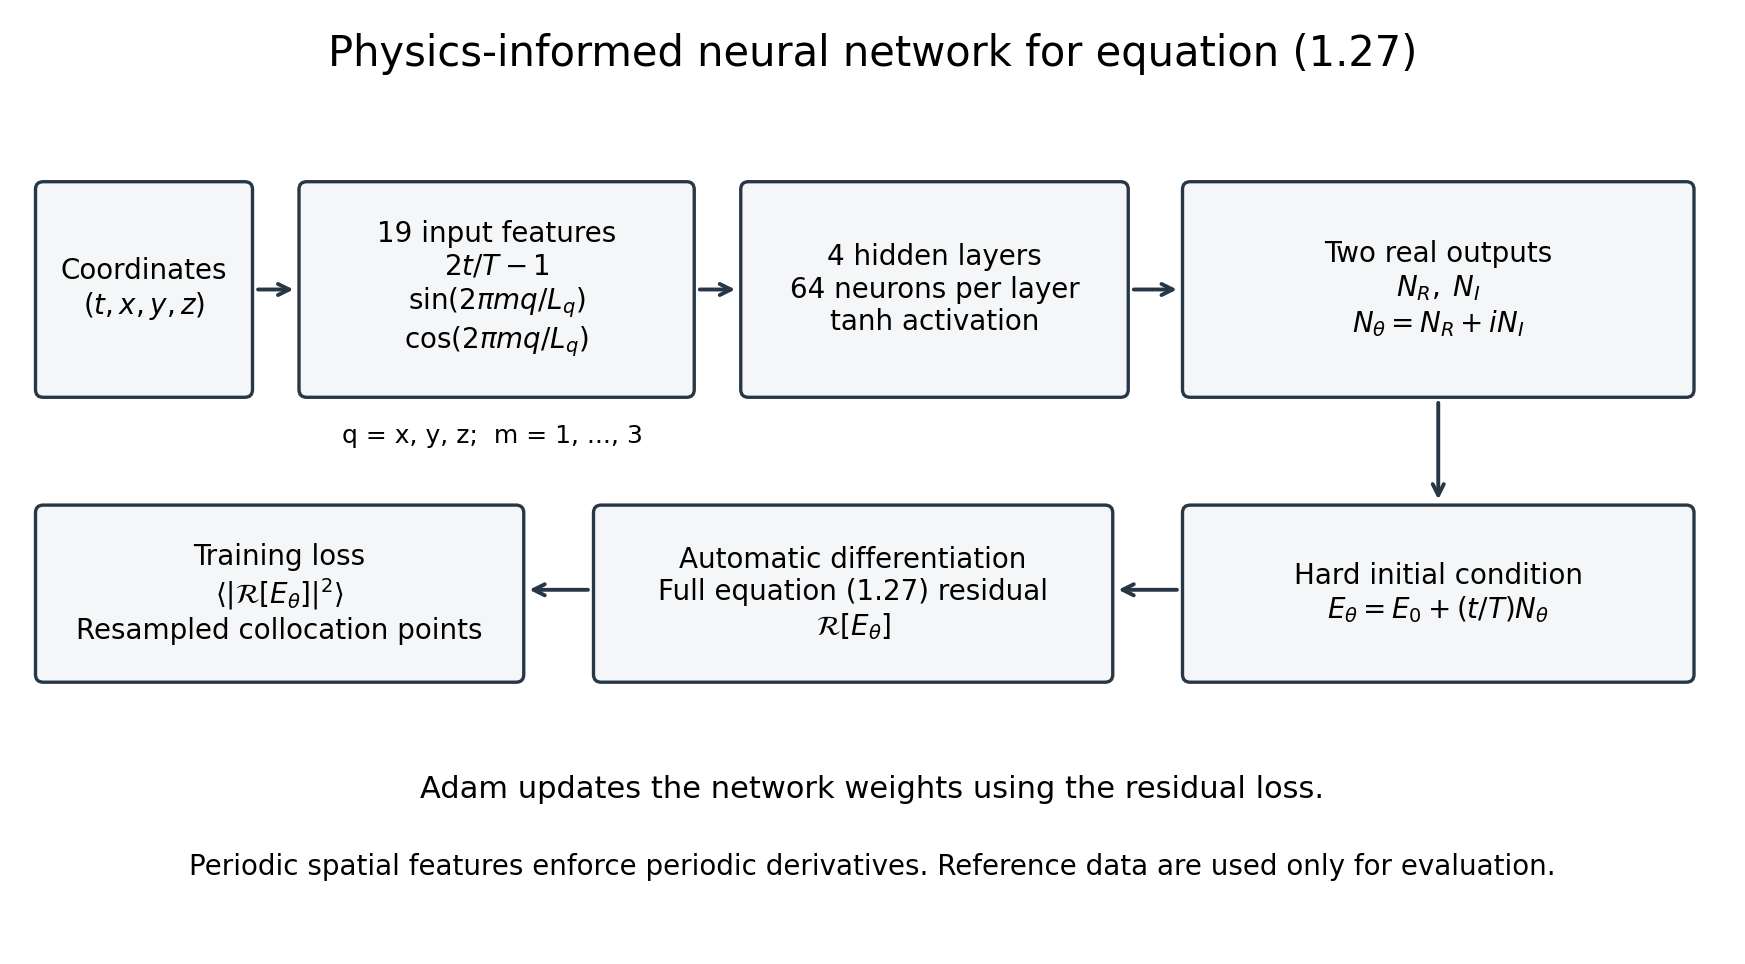
\includegraphics[width=.85\linewidth]{pinn_structure.png}\end{center}
\noindent\textbf{Figure 1.} The implemented PINN, shown schematically. Arrows show the sequence of calculations used to predict a field and form its training loss. The loss box omits an overall constant factor; the precise normalization is given in the preceding section. This network did not generate the late-time data reviewed here.

\paragraph{From coordinates to a field.}
The first transformation expresses each spatial coordinate using sine and cosine functions with three harmonics. There are $3\times3\times2=18$ spatial features and one normalized propagation feature, $2t/T-1$, giving 19 inputs to the hidden layers. These periodic features ensure that the prediction and its spatial derivatives match across opposite box faces. The network produces two real numbers, $N_R$ and $N_I$, interpreted as $N_\theta=N_R+iN_I$.

The final envelope is constructed as
\[
E_\theta(t,x,y,z)=E_0(x,y,z)+(t/T)N_\theta(t,x,y,z).
\]
At $t=0$, the correction vanishes, so the initial pulse is reproduced exactly for every choice of weights. This is a \textbf{hard initial condition}: it is built into the formula rather than merely encouraged by an additional loss term. The network learns the subsequent change in the field. $T$ is the end of its training interval.

\paragraph{Which method produced this report's data?}
The late-time results came from a Fourier numerical solver. It represents the field on a spatial grid, computes spatial derivatives through Fourier modes, and advances the equation in increments of the propagation coordinate. The fine-step run uses $\Delta t=0.01$, while the separate coarse preview uses $0.5$. It has no trainable weights, neural-network layers, or training loss. In contrast, the PINN represents the field as an adjustable function of all four coordinates and optimizes that function over a specified interval. Accordingly, the late-time oscillations in this report are not evidence of neural-network overfitting or an architectural failure.

The existing PINN has been evaluated only through $t=0.5$. The trajectory to $t=2048$ provides no new measurement of that network's accuracy. The distinction also explains why configuration entries for network width, training steps, or CUDA are not evidence that a neural network or GPU produced this reference calculation.
\clearpage
\section{Numerical experiments and available evidence}
The calculation evolves from $t=0$; the late window is not an independently restarted copy of the initial packet. The reference uses $64^3$ spatial points, strict retained modes $|m_j|<16$, and integrating-factor RK4 at $\Delta t=0.01$. There are 31 retained modes per coordinate. Scalar diagnostics have spacing $1$ in $t$; saved field frames have spacing $4$. The total simulation runtime was $5.117$ hours.

These settings describe the original fine-step run. The separate preview uses $32^3$ points and $\Delta t=0.5$, targeting $12288$ with detailed observation on $1500$--$2500$. Its stop at $10321$ and concentration results are described in the final addition. Neither run restarts the original packet at the beginning of a late observation window.
\subsection{Fine-step data and integrity checks}
The reviewed inputs are the submitted \texttt{summary.json} and \texttt{settings.json} in \texttt{results/\allowbreak late-window-\allowbreak 1024-2048}, commit \texttt{599d25b}. Their configurations agree. All diagnostic entries are finite, times are exactly $0,1,\ldots,2048$, step numbers agree with $\Delta t$, and recorded extrema of mass drift and spectral-edge fraction agree with recomputation from the rows. Status is \texttt{completed\_unvalidated}; zero steps remain.

The summary reports 257 saved frames, but neither the field archive nor the numerical checkpoint was pushed. Consequently this review cannot independently verify those frames, reconstruct three-dimensional structure, inspect phase, or recompute spectral diagnostics from the fields. The inherited configuration contains CUDA and training entries, but this run uses the NumPy reference solver and does not train or evaluate a PINN. Hardware and executed source revision are not recorded in the submitted run summary.
\clearpage
\section{Observed peak dynamics}
\begin{center}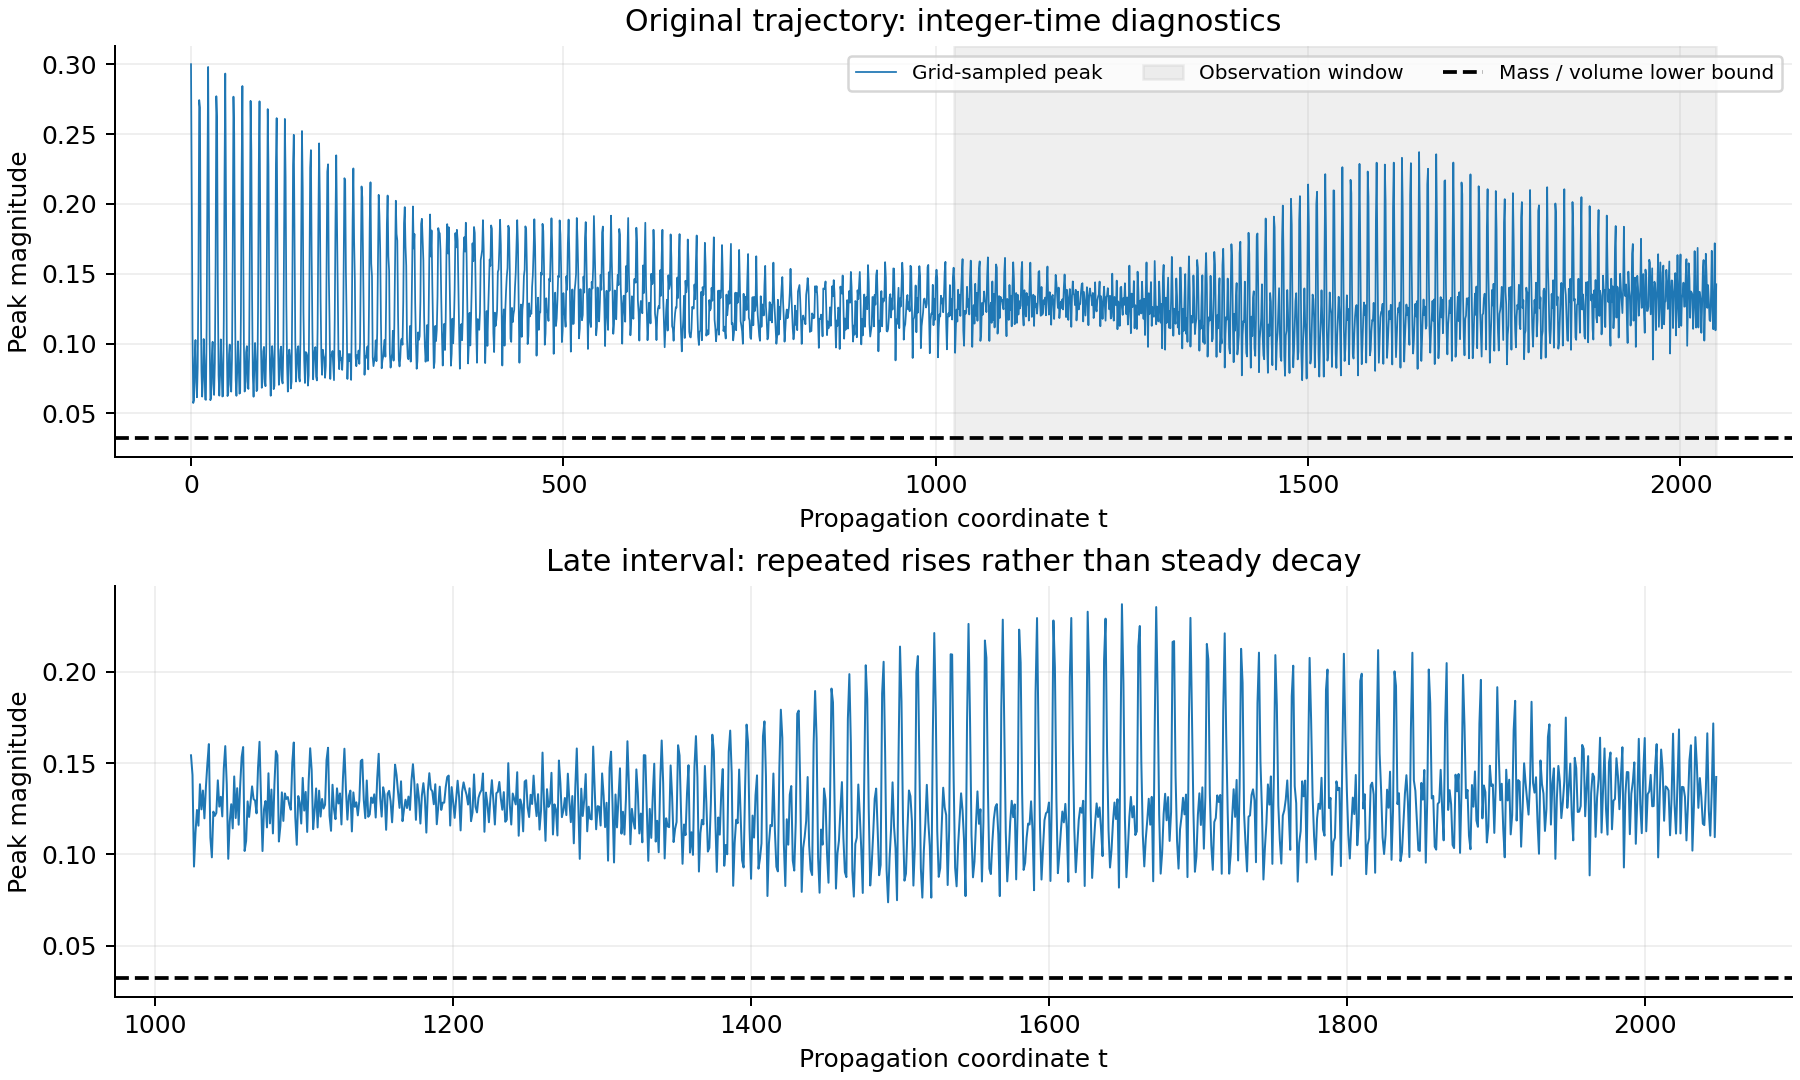
\includegraphics[width=\linewidth]{peak_history.png}\end{center}
\noindent\textbf{Figure 2.} Peaks computed on the spatial grid at integer propagation times. Shading marks the late observation interval. The dashed lower bound follows from the conserved integral and box volume; it is not a fitted curve. Connecting lines do not establish behavior between samples.

On $1024\leq t\leq2048$, the minimum is $0.0737686$ at $t=1492$ and the maximum is $0.237073$ at $t=1649$, a ratio of approximately $3.21$. The mean is $0.130717$ and median $0.127753$. The final peak is $0.142427$, compared with the initial peak $0.3$. A smaller endpoint than the initial value does not establish monotonic or asymptotic decay.
\begin{center}\small\begin{tabular}{rrrrrr}\toprule
Interval & $n$ & Mean & Minimum & Maximum & Fitted $\alpha$\\\midrule
1024--1280 & 256 & 0.13000 & 0.09336 & 0.16170 & -0.031 \\
1280--1536 & 256 & 0.12529 & 0.07377 & 0.22128 & 0.239 \\
1536--1792 & 256 & 0.13272 & 0.07717 & 0.23707 & -0.464 \\
1792--2048 & 257 & 0.13484 & 0.08853 & 0.21193 & -0.170 \\
\bottomrule\end{tabular}\end{center}
\noindent The first three intervals are half-open; the final interval includes $2048$. Statistics therefore do not double-count shared endpoints. The fitted slopes change sign. The late behavior is consistent with persistent oscillatory dynamics; exact recurrence, localization, and soliton structure cannot be diagnosed from peaks alone.
\clearpage
\clearpage
\section{A descriptive fit to the rapid oscillations}
The late peak contains repeated sharp rises and falls. A single sinusoid does not describe their shape well. To visualize this structure, the interval $1536\leq t\leq1664$ is fitted with a slowly varying baseline and four harmonics:
\[
\widehat P(t)=c_0+c_1\tau+
\sum_{k=1}^{4}\left[(a_k+b_k\tau)\cos(2\pi kfu)
+(d_k+e_k\tau)\sin(2\pi kfu)\right],
\qquad u=t-1600,\quad\tau=u/64.
\]
A harmonic is an oscillation at an integer multiple of a base frequency. Combining harmonics allows sharper peaks than one sine wave; the linear amplitude factors allow their height to change across this local interval. The 18 linear coefficients are fitted by least squares, while the base frequency is optimized in $0.084\leq f\leq0.091$, guided by the sampled spectrum. This frequency interval is a modelling choice, not a physical constraint.
\begin{center}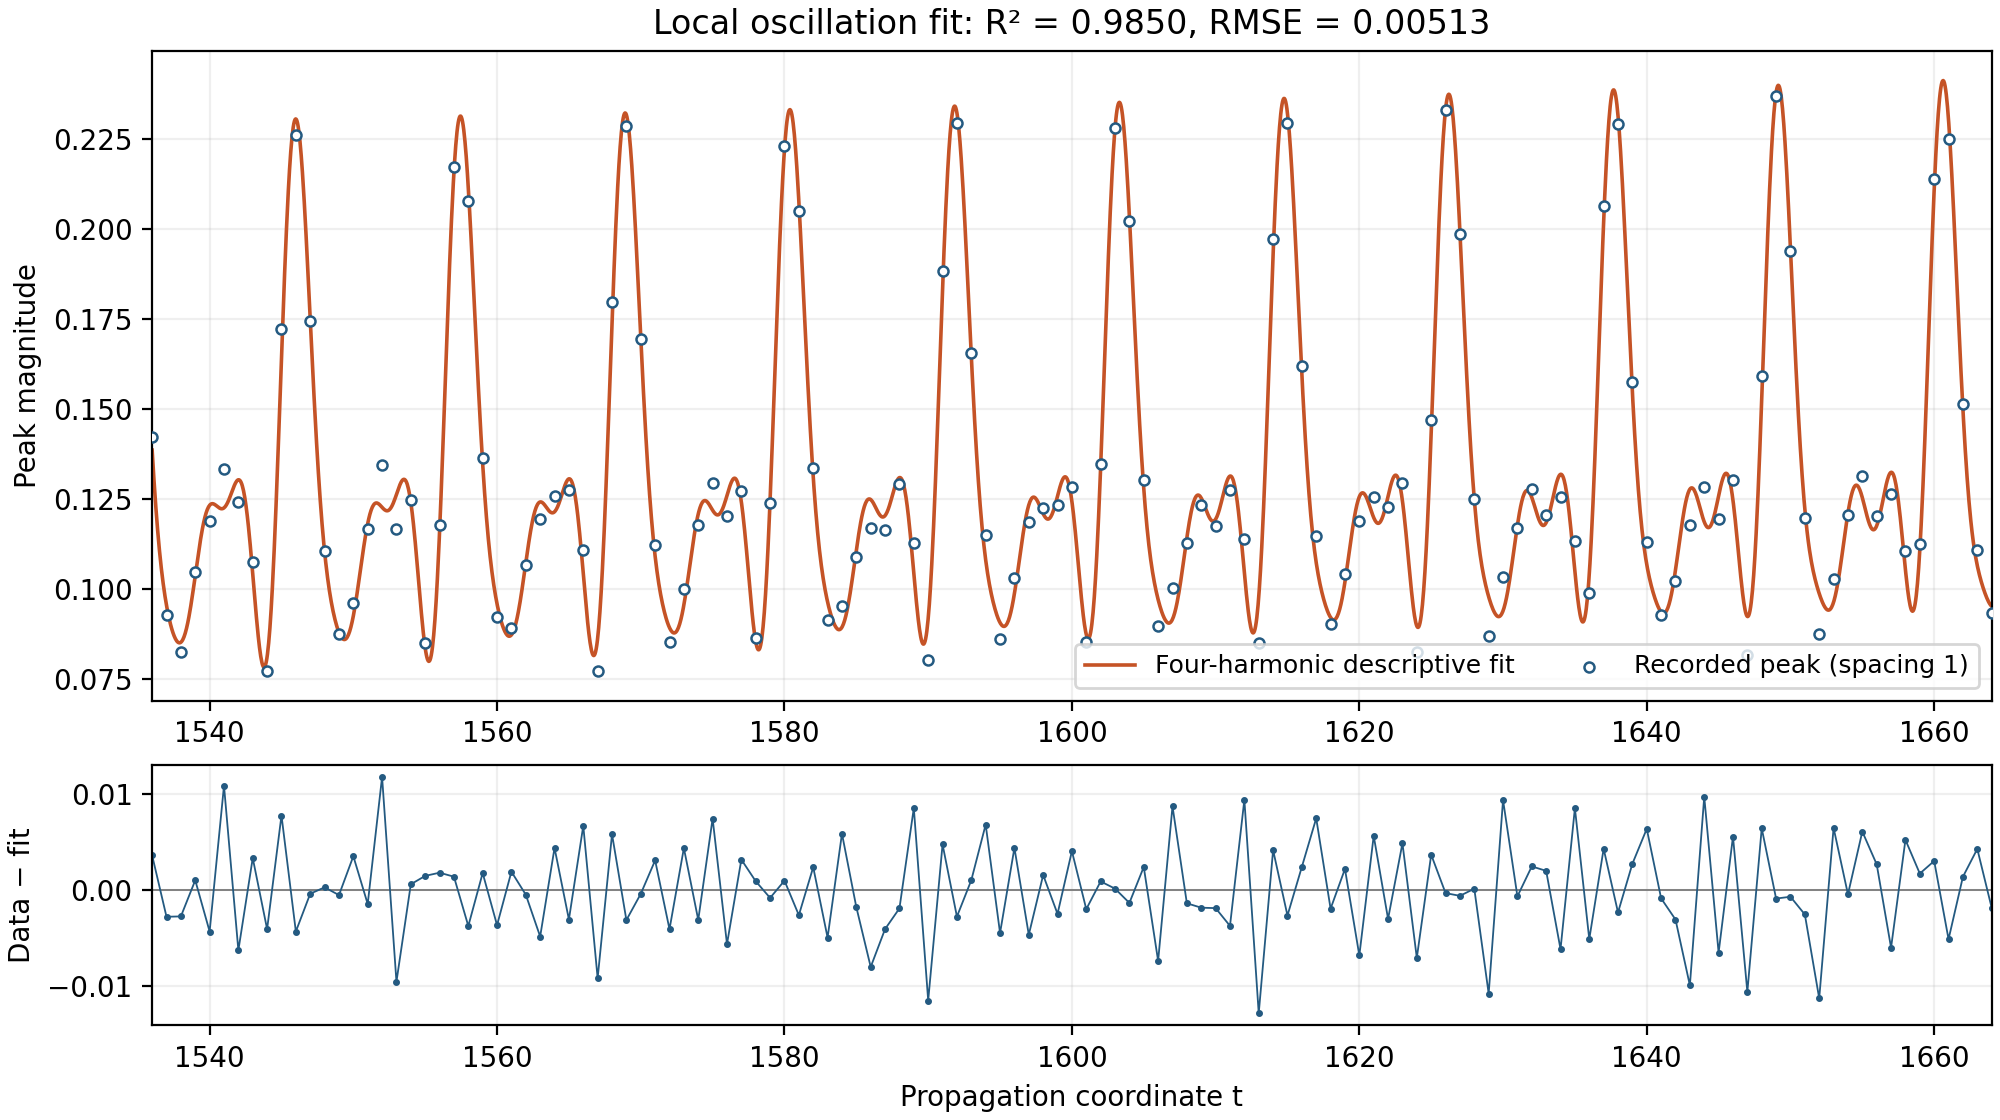
\includegraphics[width=\linewidth]{oscillation_fit.png}\end{center}
\noindent\textbf{Figure 3.} Recorded peak values and the local oscillatory fit, with residuals beneath. The smooth line approximates the sampled data; it is not a new PDE solution or a prediction outside this interval.

The fitted base period is $11.4821$, and its second harmonic has period $5.7411$. The refit on all 129 points has RMSE $0.00513$ and $R^2=0.9850$. These quantify local descriptive agreement, not long-time numerical accuracy.

Harmonic counts one through four were compared by withholding every fifth point. Their validation RMSEs were $0.03474$, $0.01802$, $0.00870$, and $0.00523$, respectively. Four harmonics were selected and then refitted using all points. Because these withheld points selected the model, they are not an independent final test. The fit uses 19 adjustable quantities including frequency. Sampling at unit intervals cannot rule out aliased higher frequencies or establish the exact continuous peak between records. Neither the fitted periods nor the high local $R^2$ establish a soliton, a decay exponent, or a globally periodic orbit.

\clearpage
\section{Upper and lower modulation traces}
\begin{center}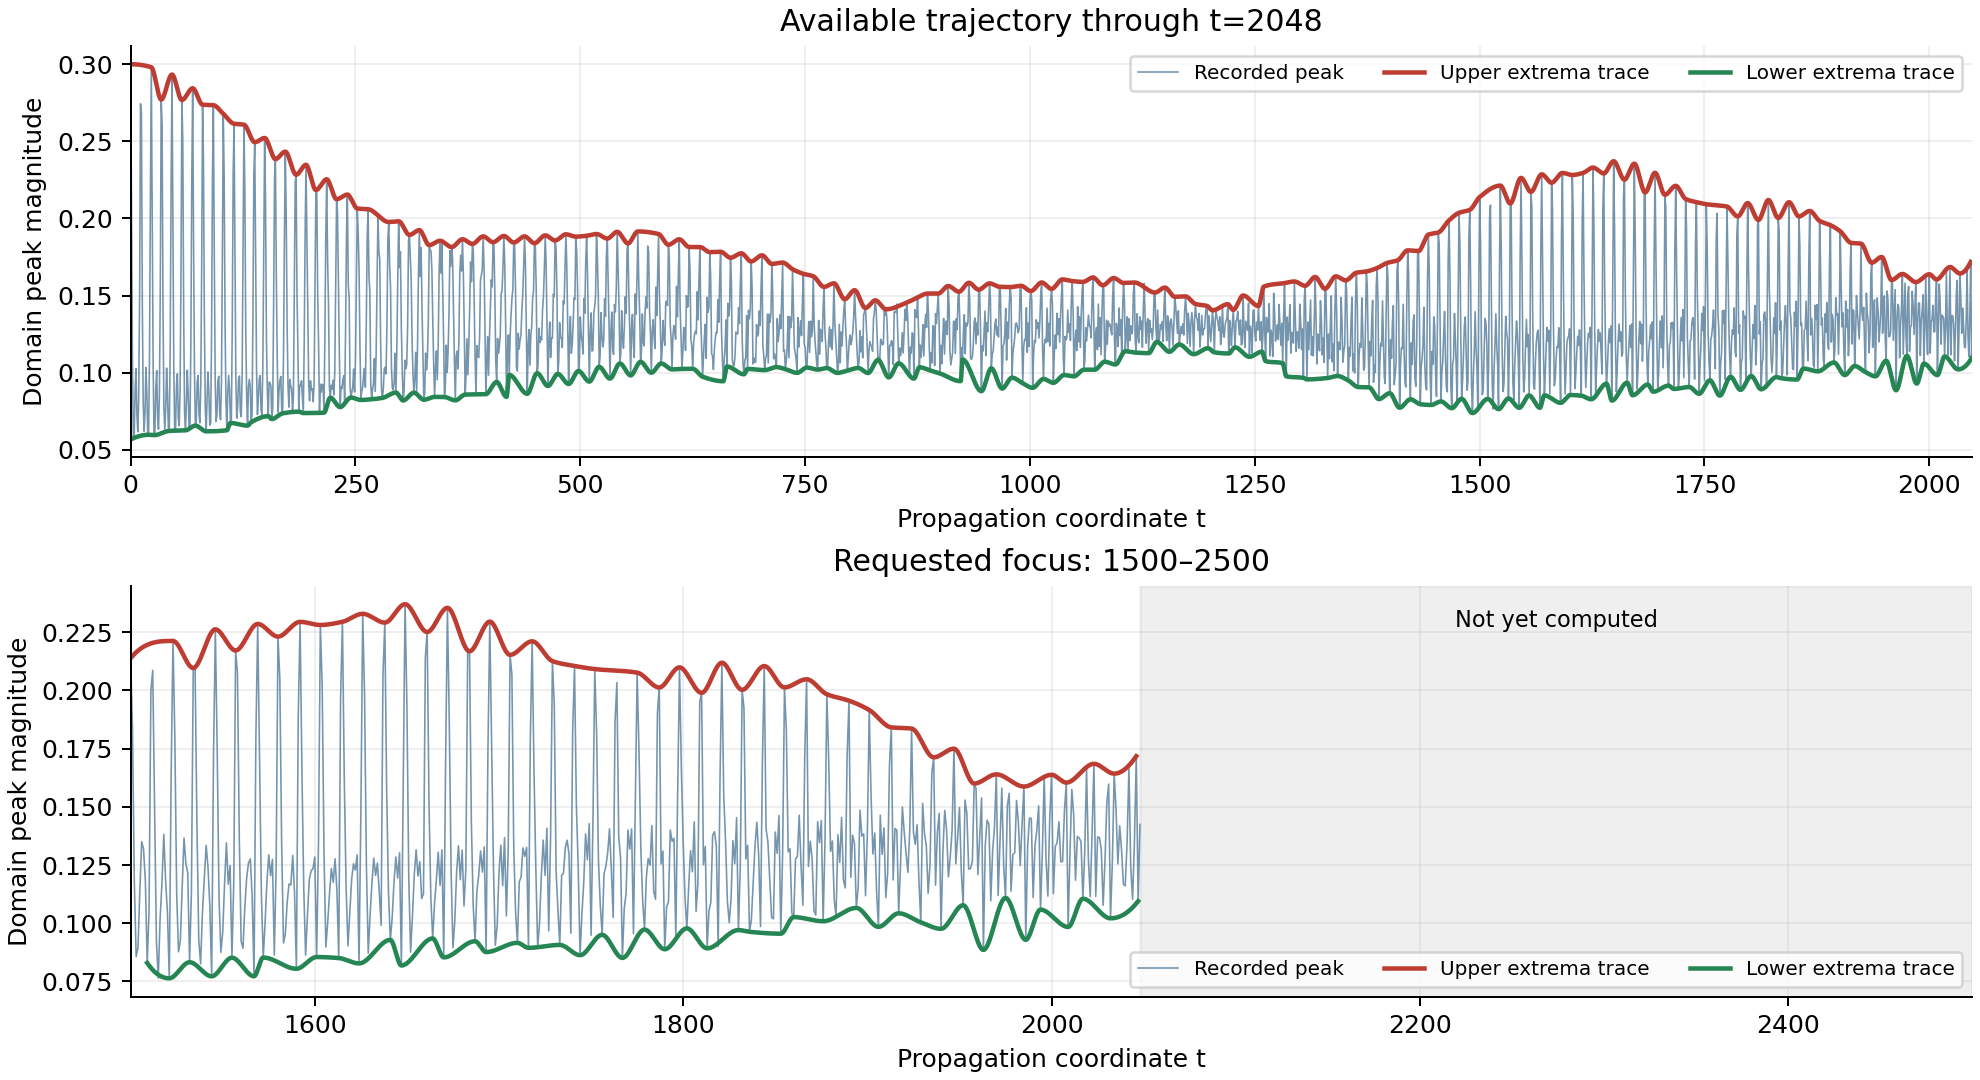
\includegraphics[width=\linewidth]{peak_envelopes.png}\end{center}
\noindent\textbf{Peak envelopes.} Red and green curves trace the maximum and minimum in successive 12-unit intervals using shape-preserving cubic interpolation. This bin length approximates the fitted base oscillation period. These descriptive traces are not guaranteed mathematical bounds; binning and temporal sampling can miss extrema. They do not extrapolate past available observations.

The separation between the traces highlights slow changes in oscillation amplitude. Around $t=1500$--$1750$, the upper peaks rise while the lower trace stays substantially lower. This is consistent with stronger modulation, but does not by itself show that a localized pulse narrows and widens. Spatial width, concentration, and phase are absent from this submitted dataset.

The requested focus is $1500\leq t\leq2500$. The shaded region after $2048$ is deliberately left without data because this fine-step trajectory ends there. The separate coarse preview covers the full focus interval and supplies concentration measures and thousand-point showcases later in this report. Its samples are not spliced into this figure because its grid and time step differ.

\clearpage
\section{Numerical reliability: what passed and what did not}
\begin{center}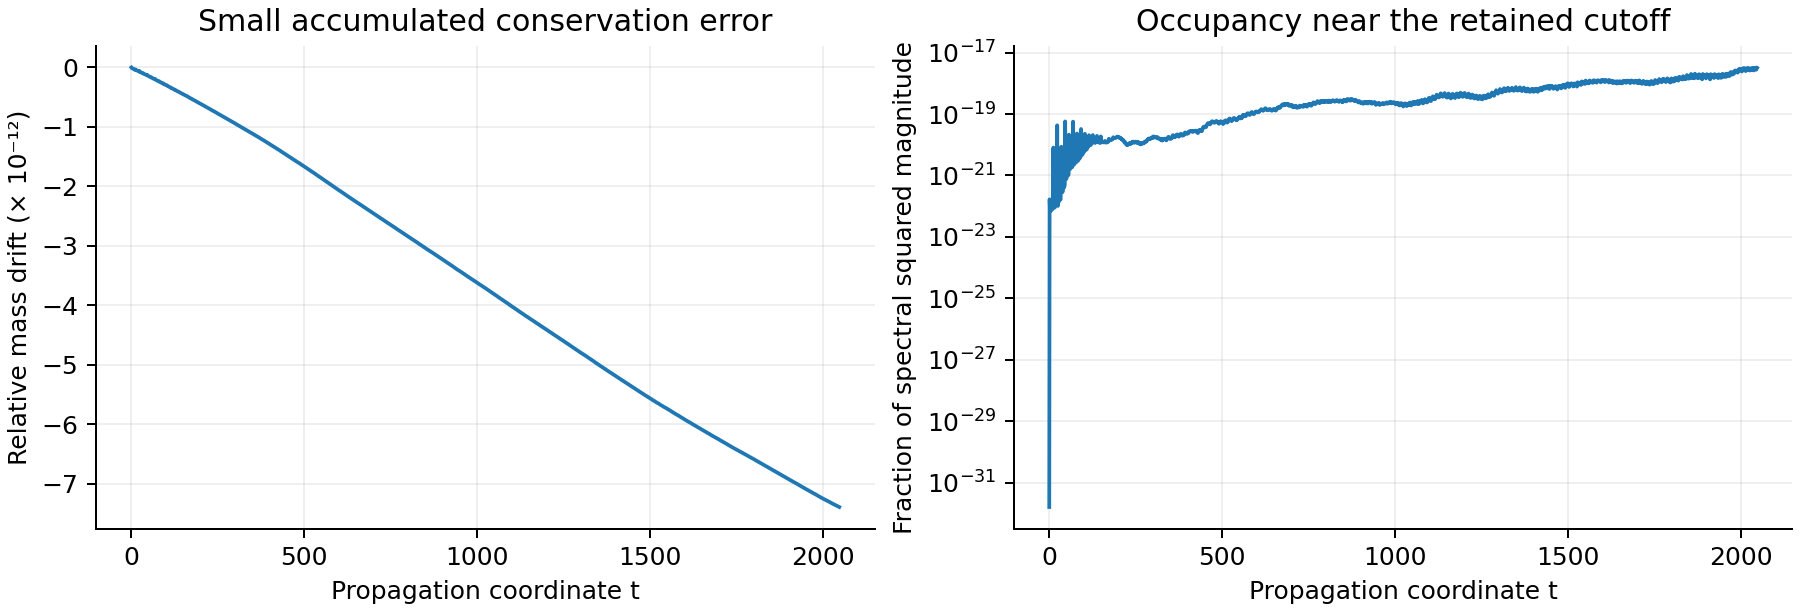
\includegraphics[width=\linewidth]{diagnostics.png}\end{center}
\noindent\textbf{Figure 4.} Conservation and high-mode occupancy over the full trajectory. Neither diagnostic compares this trajectory with an independently refined one.

Let $M_h=\Delta V\sum |E|^2$. The initial value is $1.785345681310$ and the final value is $1.785345681297$. The maximum relative drift is $7.39085\times10^{-12}$, far below the $10^{-3}$ operational stop threshold. This is excellent numerical conservation, not a $10^{-11}$ bound on solution error. A phase-shifted field can have identical mass and a large complex-field error.

The largest spectral-edge fraction is $3.27698\times10^{-18}$. The code measures energy in retained modes outside the inner region $|m_j|<12.8$. Thus the numerator includes retained modes with some coordinate magnitude $13$, $14$, or $15$. This suggests that the retained solution has little activity near the cutoff. The algorithm explicitly removes modes $|m_j|\geq16$; low edge occupancy is a useful diagnostic, not a direct measurement of all omitted spectral content.

The initial projection error is $3.56\times10^{-16}$, as expected for this low-degree trigonometric packet. No long-time $\Delta t/2$ or spatial refinement was supplied. In the earlier $T=8$ test, the $32^3$--$64^3$ peak difference reached $0.795\%$, exceeding the $0.5\%$ threshold, even though complex-field agreement was much better. The present run does not resolve that failure. A sampled maximum can change when its location falls between grid points; Fourier interpolation and a refined comparison are needed to separate peak sampling error from evolution error.

The periodic box also limits interpretation independently of numerical accuracy. Waves can repeatedly interact through the boundaries. The observed oscillations are compatible with such dynamics, but the available scalar data do not identify their mechanism.
\section{Provisional verdict}
Execution and internal consistency pass. Conservation and retained spectral occupancy are encouraging. Long-time field accuracy, peak accuracy, continuum resolution, and physical calibration remain unestablished. The appropriate label is a completed exploratory periodic trajectory, not a validated late-time reference for PINN training or theorem testing.
\clearpage
\section{Decay inequalities and the fixed-box obstruction}
For a smooth periodic solution with conserved $M=\int_\Omega|E|^2\,dV>0$, elementary integration yields
\[
M\leq |\Omega|\|E(t)\|_\infty^2,
\qquad \|E(t)\|_\infty\geq\sqrt{M/|\Omega|}.
\]
Here $|\Omega|=12^3=1728$, giving the positive lower bound
\[
\|E(t)\|_\infty\geq 0.0321432.
\]
The same inequality holds algebraically for $P_h=\max|E|$ and $M_h$ on a uniform grid. Mass conservation for (1.27) follows by periodic integration by parts: the linear Fourier multiplier is purely imaginary, the local cubic term contributes no real change to $M$, and the derivative cubic term integrates to a derivative of $|E|^4$. This argument assumes sufficient regularity.

Therefore a nonzero fixed-box solution cannot obey $P(t)\leq Ct^{-\alpha}$ for all sufficiently large $t$ with finite $C$ and $\alpha>0$. The current oscillations are not a counterexample to a whole-space estimate: its domain, hypotheses, norm, and constants must first match the experiment. On any finite time interval, a bound with freely chosen sufficiently large $C$ is not disproved by a rebound.
\begin{center}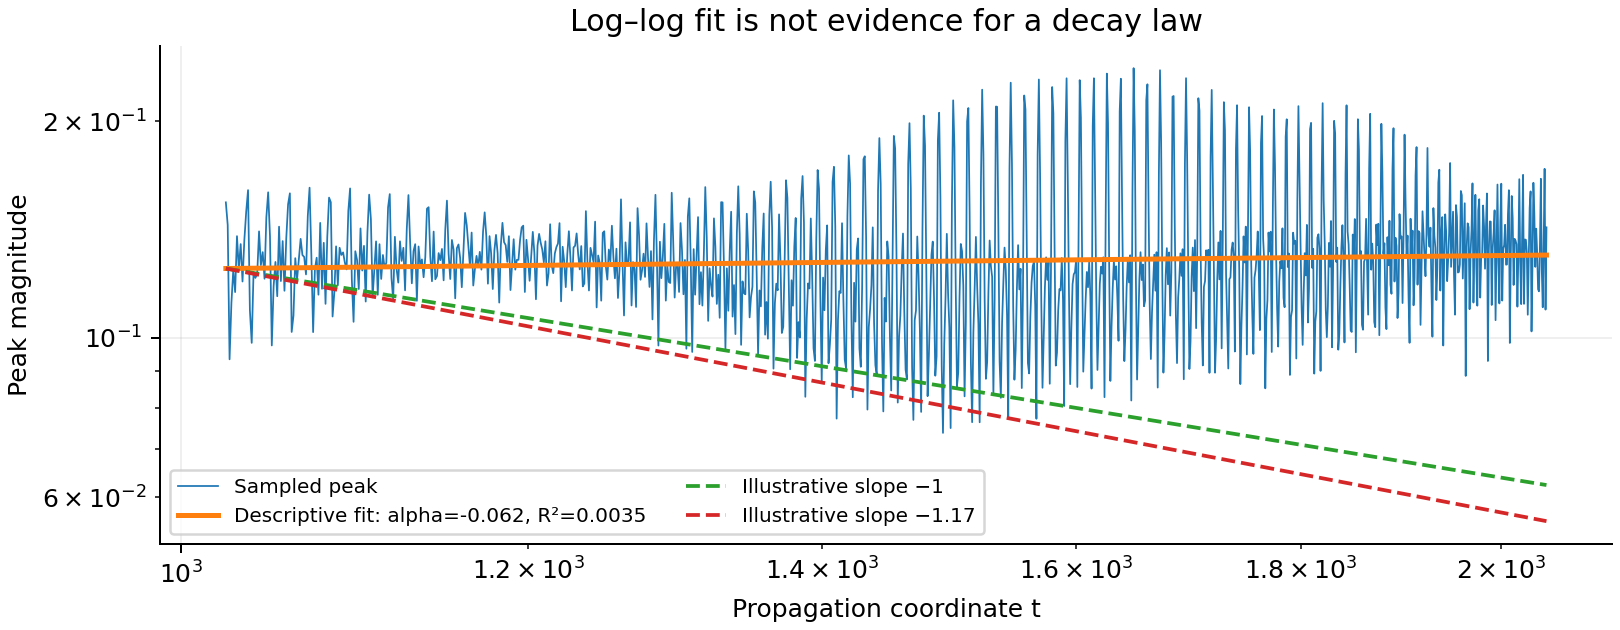
\includegraphics[width=\linewidth]{fit.png}\end{center}
\noindent\textbf{Figure 5.} Ordinary least squares of $\log P_h$ against $\log t$ on integer samples $1024$ through $2048$. The comparison slopes $-1$ and $-7/6$ are illustrative and normalized to the fitted curve at $1024$; they are not imported claims about this periodic solution.

The fitted $\alpha=-0.0620$ is slightly negative and $R^2=0.00351$ is very small. This describes an oscillatory finite record; it does not establish growth or a sharper decay exponent. Subinterval slopes are unstable, and serially dependent deterministic samples do not justify ordinary independent-sample confidence intervals. The time span covers only a factor of two in $t$.
\paragraph{Reproducibility.} The source bundle includes submitted JSON inputs, recomputed statistics, analysis code, figures, and this LaTeX source. The source summary hash is recorded in \texttt{review-statistics.json}. This review computes no new long-time PDE solution and makes no experimental-data validation claim.
\clearpage
\section{Addition: results of the coarse breathing preview}
This addition reviews the newly submitted $32^3$, $\Delta t=0.5$ reference run, commit \texttt{b12b69c}. It uses the same equation, initial pulse, and periodic box as the main report. It is a separate calculation, not an extension of the previously reviewed $64^3$ trajectory, and no PINN was trained.
\begin{center}\small\begin{tabular}{lr}\toprule
Quantity & Recorded result\\\midrule
Target / reached propagation & $12288$ / $10321$\\
Elapsed execution time & $121.24$ seconds\\
Integration steps / reported saved frames & $20642$ / $726$\\
Maximum relative mass drift & $1.000073\times10^{-3}$\\
Maximum spectral-edge fraction & $2.65135\times10^{-6}$\\
Status & \textnormal{failed\_diagnostics}\\\bottomrule\end{tabular}\end{center}
The run stopped at the first recorded crossing of the $0.1\%$ mass-drift threshold. Mass increased numerically; this is a conservation error, not evidence of physical amplification. The spectral-edge threshold did not trigger. The complete $1500$--$2500$ observation interval was reached, as were the showcases through $10000$; $11000$ and $12000$ were not reached.
\begin{center}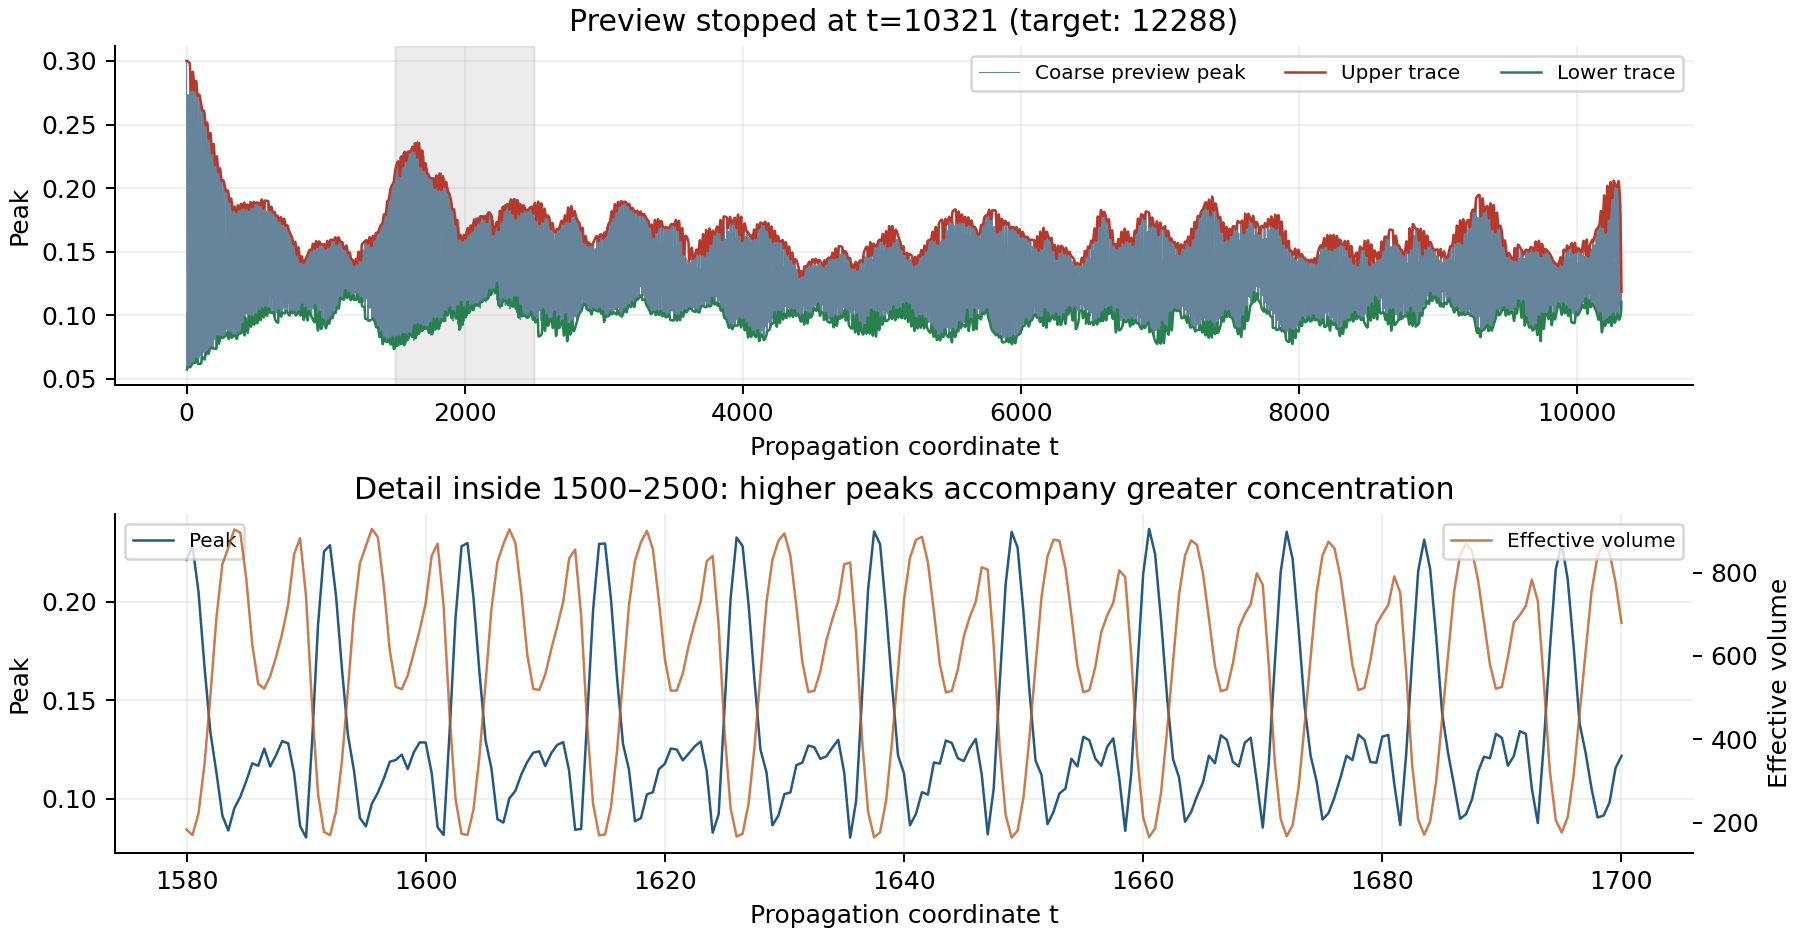
\includegraphics[width=\linewidth]{preview_results.png}\end{center}
\noindent\textbf{Preview Figure A.} The available long trajectory with upper and lower extrema traces, followed by a detail showing peak height and effective volume on separate vertical scales. Extrema traces interpolate maxima and minima in 12-unit bins and are descriptive, not rigorous bounds. The shaded interval is $1500$--$2500$.
\clearpage
\section{Concentration and thousand-point showcases}
Over $1500\leq t\leq2500$, the 2,001 diagnostic samples have peak magnitudes between $0.073723$ and $0.236918$. The effective volume
\[
V_{\mathrm{eff}}=\frac{\left(\int |E|^2\,dV\right)^2}{\int |E|^4\,dV}
\]
ranges from $164.37$ to $924.41$; smaller values indicate a more concentrated field. Peak and effective volume have Pearson correlation $-0.9134$ across this interval. This is a descriptive association between temporally dependent samples, not an independent-sample significance test or evidence of causation.

The highest recorded focus-window peak occurs at $t=1660.5$, with $V_{\mathrm{eff}}=165.17$. Thus this preview provides more evidence for repeated concentration and spreading than the peak-only data did. However, 338 of 2,001 focus samples ($16.9\%$) have at least one weak circular centroid, making the corresponding width difficult to interpret. A single coherent localized breather is not established. The effective-volume measure is independent of the centroid choice, but it too cannot distinguish all possible multi-pulse structures.
\begin{center}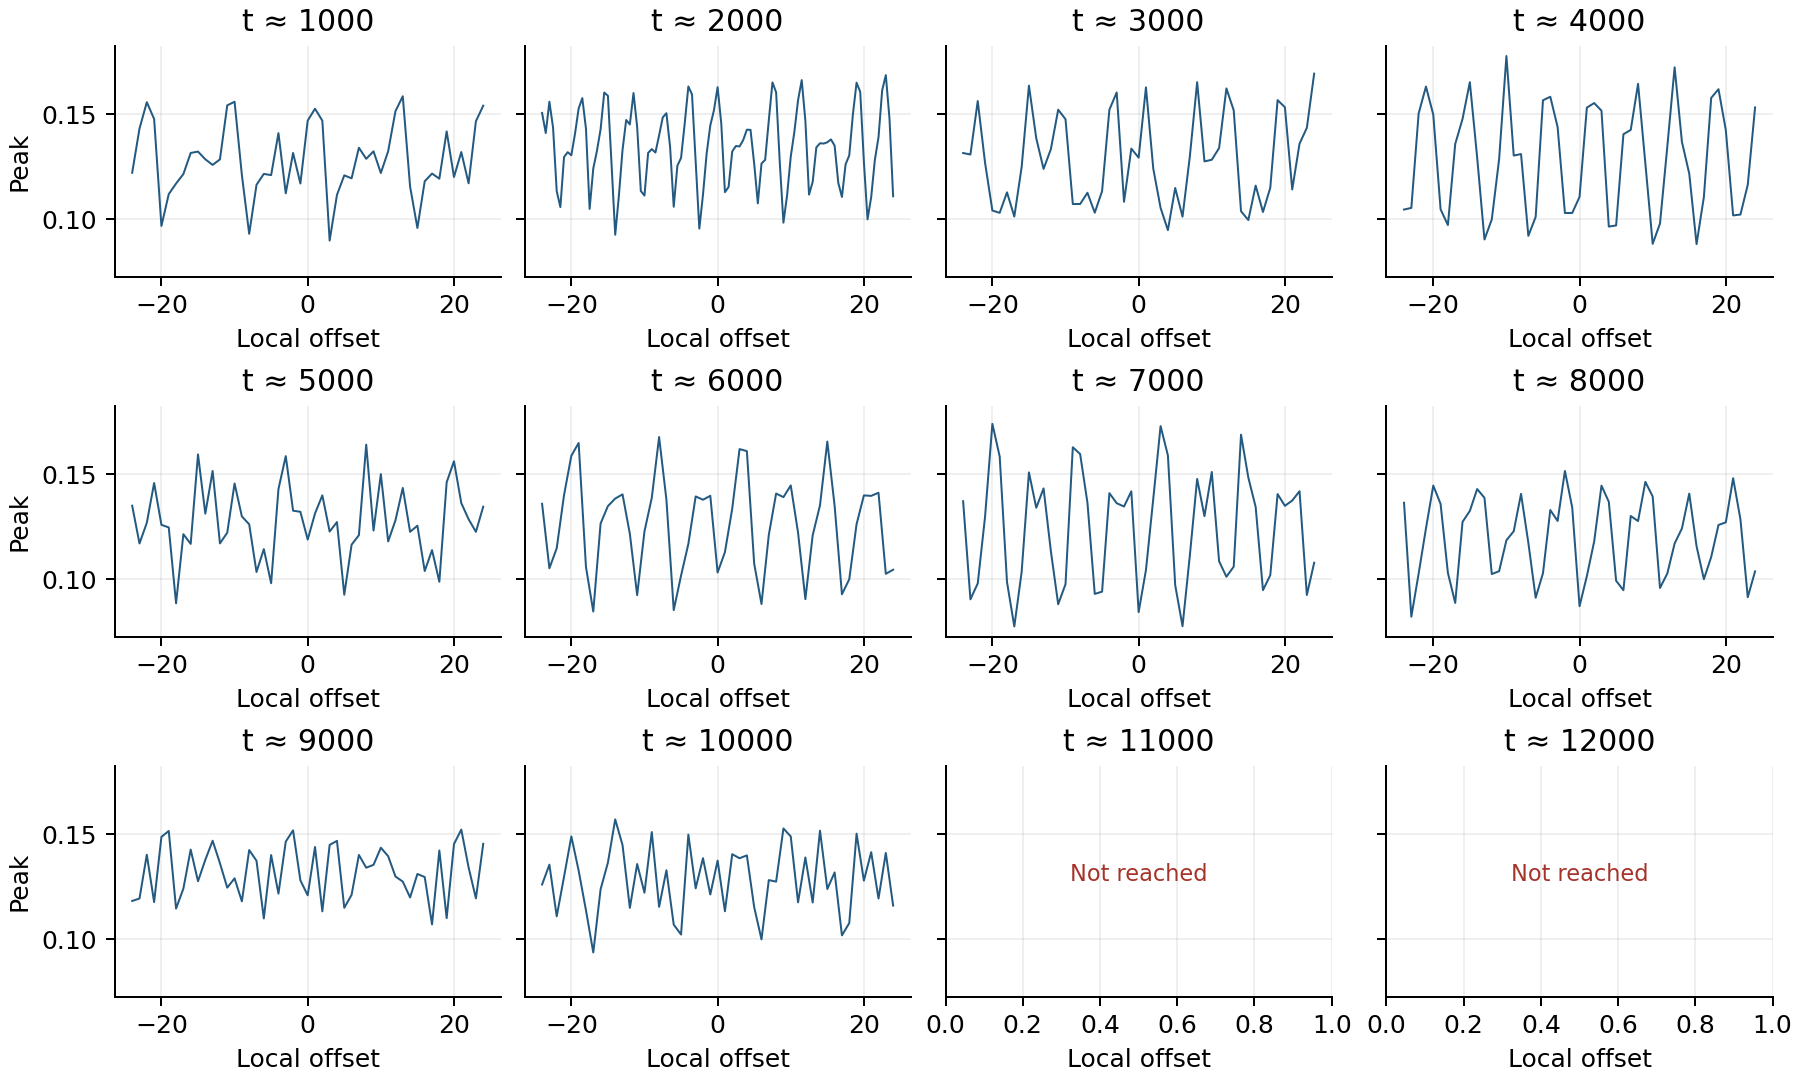
\includegraphics[width=\linewidth]{preview_milestones.png}\end{center}
\noindent\textbf{Preview Figure B.} Peak histories within $\pm24$ of each thousand. All panels share the vertical scale. These are scalar histories, not spatial pulse images; the last two requested windows were not reached.

On the common integer times $1500$--$2048$, the coarse preview differs from the earlier $64^3$, $\Delta t=0.01$ result in sampled peak by at most $1.04\%$, with mean relative discrepancy $0.223\%$. This is useful overlap agreement, but it combines grid and step changes and does not validate the complex field or the trajectory beyond $2048$. Focus-window mass drift reaches $0.0190\%$, below the operational stop threshold; passing that check alone does not establish field accuracy.

Only the summary and settings were supplied, so spatial shape, phase, and the reported field-frame files were not independently inspected. The result is a successful inexpensive qualitative preview that terminated on a numerical diagnostic, with breathing-like concentration modulation rather than a demonstrated breather or a decay law.

\end{document}
